\section{Out-of-Distribution Actions in Q-Learning}
\label{sec:Problem Description}

% Q-learning and other ADP methods which rely on iterating the Bellman backup operator are particularly susceptible to out-of-distribution inputs, because any errors incurred on these inputs can be propagated to neighbor states via the backup and keep compounding over iterations of the algorithm. Unfortunately, error on a single state can propagate to other states and can potentially cause inaccurate predictions across the entire Q-function. As we will show, these inaccuracies do affect the performance of off-policy algorithms in practice.

When Q-learning and off-policy actor-critic algorithms are used with static off-policy data, it's common to see returns improve at first and then deteriorate, or even deteriorate right from the start, as shown in Figure \ref{fig:divergence}. At first glance, this resembles overfitting, but increasing the size of the static dataset does not rectify the problem, suggesting the issue is more complex.
%When running Q-learning on a static off-policy dataset, we often find that the performance of the algorithm is poor and the performance doesn't change drastically through training (e.g., results for the na\"{i}ve RL method in Figure \ref{fig:divergence}) whereas the Q-values usually diverge over the course of training. However, unlike in supervised learning, increasing the size of the static off-policy dataset does not rectify the problem, suggesting the situation is more complex.
%These results suggest a form of overfitting, however, the situation is more complex than supervised learning. 
%as the ground truth performance curves resemble validation error curves during overfitting in supervised learning. 
%However, this interpretation does not tell the whole story: 
%while we can test for overfitting using the Bellman error, early stopping on Bellman error is ineffective [either cite something or add an experiment on this to the appendix].
% . , suggesting that simple overfitting is an inadequate explanation. 
\begin{wrapfigure}{r}{0.5\textwidth}
\vspace{-10pt}
\begin{center}
    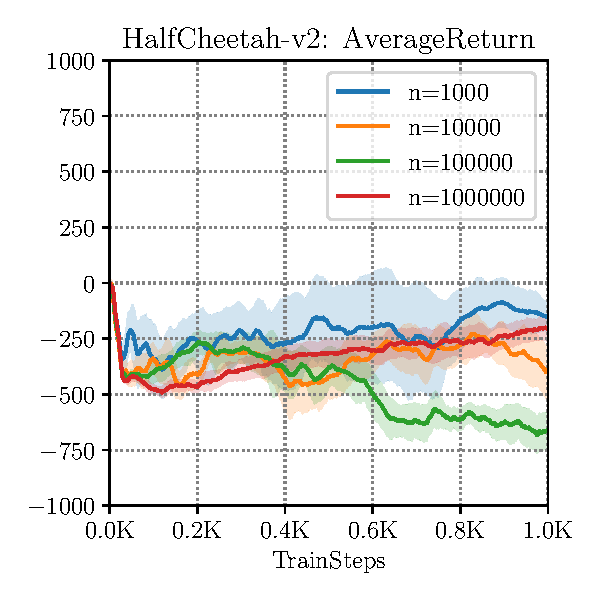
\includegraphics[width=0.48\linewidth]{images/cheetah_divergence.pdf}
    ~
    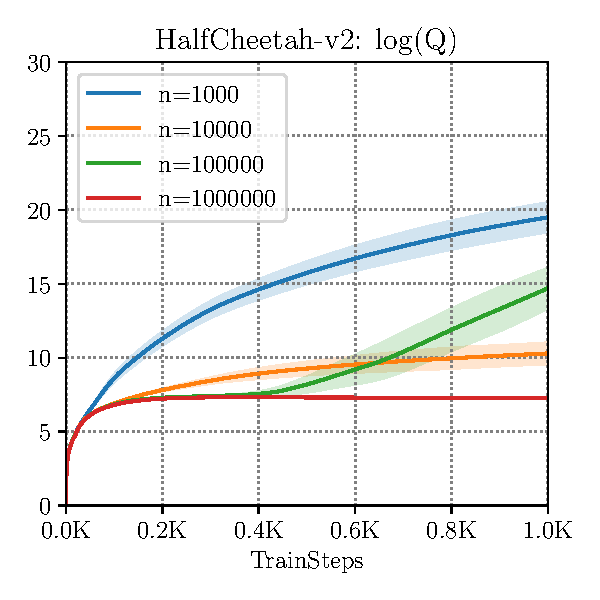
\includegraphics[width=0.48\linewidth]{images/cheetah_divergence_q_val.pdf}
  \end{center}
 \vspace{-10pt}
 %%SL.5.22: Very important: the y-axes are not labeled right now, and it took me a while to figure out which plot was showing what. What is log(Q)? I guess you're trying to show that the right plot has Bellman error (?), while the left has performance? A couple more things: (1) always put space before ( (you often omit this space) (2) consider a caption like this (once the figures are labeled more clearly): Off-policy learning with SAC on HalfCheetah-v2 for different dataset sizes ($n$). The performance (left) does not correlate with $n$, while the Q-values (right) diverge or saturate at values far from the actual return.
  \caption{Performance of SAC on HalfCheetah-v2 with off-policy expert data w.r.t. number of training samples ($n$). Note the large discrepancy between returns (which are negative) and logarithm of Q-values (which converge to large positive values or diverge) that is not solved with additional samples.} 
 \vspace{-15pt}
 \label{fig:divergence}
\end{wrapfigure}

We can understand the source of instability by examining the form of the Bellman backup. Although minimizing the mean squared Bellman error corresponds to a supervised regression problem, the targets for this regression are themselves derived from the current Q-function estimate. The targets are calculated by maximizing the approximate $Q$-function with respect to the action at the next state. However, the $Q$-function estimator is only reliable on inputs from the same distribution as its training set. As a result, na\"{i}vely maximizing the value may evaluate the $\hat{Q}$ estimator on actions that lie far outside of the training distribution, resulting in pathological values that incur large error. We refer to these actions as out-of-distribution (OOD) actions, and we call errors due to OOD actions \textit{boostrapping errors}. This is because not only do they produce inaccurate values on the states where the backup is computed, these errors will propagate on subsequent Bellman backups. 
If $\valerr_k(s) = |Q_k(s,a) - Q^*(s,a)|$ denotes the total error at iteration $k$ of Q-learning and $\projerr_k(s, a) = |Q_k(s,a) - \backup Q_{k-1}(s,a)|$ denote the current Bellman error, we can write $\valerr_k(s) \le \projerr_k(s,a) + \gamma \max_{a'} E_{s'}[\valerr_{k-1}(s',a')]$. This means errors from $(s', a')$ are discounted, then accumulated into $Q(s,a)$ in addition to new projection errors $\projerr_k(s, a)$ being introduced on the current iteration. $\projerr$ is expected to be high on OOD states and actions
%\TODO{gjt: explain this} 
as errors at these states-action pairs are never minimized during training.
%Furthermore, these errors are propagated to other states through the backup operator.

To mitigate bootstrapping errors, we can restrict the policy/actor to ensure that they output actions that lie in the support of training distribution. 
% \TODO{Isn't that just batch constrained Q-learning? Just restricting the actions to those in the training set. -- changed to distribution: addressed}. 
This is distinct from previous work (e.g.,~\citep{fujimoto2018off}) which constrains the \emph{distribution} of the learned policy to be close to the behavior policy, similarly to behavioral cloning~\cite{Schaal99isimitation}.
While this is sufficient to ensure that actions lie in the training set with high probability, it is overly restrictive. For example, if the behavior policy is close to uniform, the learned policy will behave randomly, resulting in poor performance, even when the data is sufficient to learn a strong policy (see Figure~\ref{fig:gridworld}.
for an illustration). The key distinction is that we restrict the support of the learned policy, but not the probabilities of the actions within the support.
Restricting the actions reduces bootstrapping error as the Q-function is no more queried on OOD actions. However, it may also prevent the algorithm from converging to the optimal $Q^*$. In the next subsection, we theoretically analyze this tradeoff.


%In order to formally analyze this problem, we perform an error propagation analysis of Q-learning on the lines of Approximate Value Iteration (AVI)~\cite{munos2003errorapi} and Approximate Policy Iteration (API)~\cite{bruno2015approximate}. Let $Q_1, \cdots, Q_K$ be the value-function iterates and $\pi_1, \cdots,\pi_k$ be the policy-iterates generated when performing actor-critic based Q-learning, which a special case of API. We can express the \emph{policy evaluation error} at iteration $k$ as $\valerr_k(s, a) = |Q_k(s, a) - Q^\pi(s, a)|$, and the \emph{projection error} as $\projerr_k(s, a) = |Q_k(s, a) - \Tpi Q_{k-1}(s, a)|$. 
%Then, we have $\valerr_k(s, a) \le \delta_k(s, a) + \gamma E_{s', \pi}[\valerr_{k-1}(s', a')]$ (see Appendix~\ref{app:error_prop} for details). In other words, approximation errors $\projerr_k(s, a)$ are introduced during the projection step, discounted, and propagated to neighboring states via the backup operator. Understanding the source of the errors and controlling them is key to producing a stable algorithm.

%When using Q-function values on actions that greedily maximize the value at the next state $s'$ ($\max_{a'} Q(s', a')$) as target values for Q-learning, the maximizing action at $s'$ can potentially be very different from the distribution of actions at state $s'$ defined by dataset distribution $\dataset$. Such actions that are very unlikely to have been sampled from the dataset distribution are called out-of-distribution (OOD) actions. 
%%SL.5.20: Can we formally define what that means, instead of just saying they are called this? -- i don't think so that we can formally define OOD in general, without going into some hypothesis testing thing.
%As neural nets are known to produce inaccurate results when queried on out-of-distribution inputs -- adversarial examples~\citep{goodfellow2015advexamples} are a well-known example of this phenomenon, Q-values corresponding to OOD actions are not accurate and reliable. This also means that using such Q-values for Bellman backups tends to destabilize Q-value estimates. Empirically, we find that OOD actions are a major source of error that arise in Q-learning style ADP methods with static-datasets. The error accumulated in the Q-function due to backups from OOD actions is called \textit{boostrapping error}. In Figure~\ref{fig:gridworld}, the top row demonstrates how error can propagate between states due to the bootstrapping process. We next propose to restrict the policy $\pi$ during policy improvement step and while computing the backup, so as to limit the amount of errors incurred due to OOD actions, which we discuss in the following sections.


%%%%%%%%%%%%%%%%%%%%%%%%%% OLD: Monday 7:04 pm
% In this section, we describe how errors occurring in the Q-function due to bootstrapping errors from certain
% %%SL.5.20: This somewhat contradicts what we wrote in the related work section -- we said the Fujimoto analysis is at the level of sets, while ours is on distributions, but now we are talking about sets too?
% actions -- which we call out-of-distribution actions -- can accumulate and hurt the performance of off-policy algorithms in practice to a major extent. We start by revisiting the study of error propagation in ADP methods.
% %%SL.5.20: I think it takes us way too long to get to the point here. Can we have a more focused opening paragraph that specifically talks about what we'll be analyzing and doing?

% %%SL.5.20: Is there any way we can move this discussion to related work? I think it breaks the flow to have a little "mini related work" at the top of the technical section. Especially after such a lengthy setup, many readers will get annoyed and wonder when you'll get around to telling them what you actually do.
% We analyse off-policy static-dataset Q-learning algorithms as specific instances of approximate value iteration (AVI)~\citep{munos2003errorapi} and approximate policy iteration (API)~\citep{bruno2015approximate}. 
% %%SL.5.20: Do you really need all this API and AVI stuff? Why not keep it simple and just discuss Q-learning?

% %%SL.5.20: Maybe we should have two subsections here -- a 4.1 that starts here and explains the problem, and a 4.2 (current 4.1) that explains the solution.

% Errors encountered during Q-learning
% %%SL.5.20: Just say Q-learning...
% %\TODO{not defined yet} 
% propagate 
% between neighbor states $s'$ and $s$ when performing a Bellman backup.
% %%SL.5.20: I feel like the above sentence is just a really long-winded way to say "The Bellman backup results in compounding errors." Try to rephrase sentences to be more concise, avoid unnecessary words.
% To formalize this, let $Q_1, \cdots, Q_K$ be the value-function iterates and $\pi_1, \cdots,\pi_k$ be the policy-iterates generated when performing actor-critic based Q-learning. We can express the \emph{policy evaluation error} at iteration $k$ as $\valerr_k(s, a) = |Q_k(s, a) - Q^\pi(s, a)|$, and the \emph{projection error} as $\projerr_k(s, a) = |Q_k(s, a) - \Tpi Q_{k-1}(s, a)|$. 
% Then, we have $\valerr_k(s, a) \le \delta_k(s, a) + \gamma E_{s', \pi}[\valerr_{k-1}(s', a')]$ (see Appendix~\ref{app:error_prop} for details).
% % \TODO{all for a fixed $\pi$, how is this related to Q learning}
% % \TODO{define $V_k$, etc.}
% In other words, approximation errors $\projerr_k(s, a)$ are introduced during the projection step, discounted, and propagated to neighboring states via the backup operator. Understanding the source of the errors and controlling them is key to producing a stable algorithm.
% %%SL.5.20: This seems like a reasonable statement, but I think readers will be lost at this point about where you are going. Maybe you can preface the above paragraph by saying something like this: When training on off-policy data, we often see actual policy performance improving briefly and then deteriorating sharply (see, e.g., results for the na\"{i}ve RL method in Figure ???). One might at first surmise that these issues are a form of overfitting, as the ground truth performance curves resemble validation error curves during overfitting in supervised learning. However, this interpretation does not tell the whole story: while we can test for overfitting using the Bellman error, early stopping on Bellman error is ineffective [either cite something or add an experiment on this to the appendix]. Furthermore, even a very large off-policy training set does not avoid this degradation problem, suggesting that simple overfitting is an inadequate explanation. We can obtain a better explanation from examining the form of the Bellman backup. Note that minimizing the Bellman error corresponds to a supervised regression problem, but the targets for this regression are themselves derived from the current Q-function estimate. We argue that it is these estimates themselves that are the sources of the degradation: they are calculated by finding the action that maximizes the value at the next state. However, the value estimate is obtained from a function approximator, and this function approximator is only reliable on inputs from the same distribution as its training set. Since Q-learning only trains the Q-function via regression on state-action tuples seen in the training data, the actions that maximize the target value might lie very far outside of the training distribution, and therefore might incur very large error. We can formally analyze this source of error as follows. [and then talk about delta etc]

% These errors $\valerr_k$ arise from a multitude of sources and include function approximation error, sampling error, distribution shift error, and bootstrapping error. When learning from static, off-policy datasets, sampling error is largely uncontrollable, and it is hard to provide guarantees about function approximation error with deep neural nets.
% %%SL.5.20: I think this is misleading. While it's true that we cannot provide guarantees, in general function approximation error with large function approximators is low. You can reference our debugging paper for this.
% When training Q-functions using $(s, a, r, s')$ tuples from the dataset, the fixed point iteration scheme
% %%SL.5.20: Which fixed point iteration scheme?
% queries and uses the Q-function value on actions that greedily maximize the value at the next state $s'$ ($\max_{a'} Q(s', a')$). However, the maximizing action at $s'$ can potentially be very different from the distribution of actions at state $s'$ defined by dataset distribution $\dataset$. Such actions that are very unlikely to have been sampled from the dataset distribution are called out-of-distribution (OOD) actions.
% %%SL.5.20: Can we formally define what that means, instead of just saying they are called this?
% Neural nets are known to produce inaccurate results when queried on out-of-distribution inputs -- adversarial examples~\citep{goodfellow2015advexamples} are a well-known example of this phenomenon.
% %%SL.5.20: That's a good explanation
% Regressing to the target-value computed using such OOD actions coupled with the $\max$ step can lead to an accumulation of error in the Q-function by virtue of error propagation.
% %%SL.5.20: Now it's again unclear whether you are talking about the same phenomenon, or something else. Basically, the logical connection between the sentence "Neural nets.." and "Regressing.." is missing.
% %\TODO{is $\pidata$ a single policy or set? -- set}.
% The problem is further exacerbated by the fact that updates are only made to Q-values of state-action pairs present in $\dataset$, so even though the Bellman backup queries the Q-function for OOD actions, it never \emph{trains} it on those actions. As deep neural-net function approximators can often generalize in undesired and unpredictable ways, such backups can destabilize learning and can lead to divergence in Q-functions.

% Empirically, we find that OOD actions are a major source of error that arise in Q-learning style ADP methods with static-datasets. The error accumulated in the Q-function due to backups from OOD actions is called \textit{boostrapping error}. In Figure~\ref{fig:gridworld}, the top row demonstrates how error can propagate between states due to the bootstrapping process.
% %%SL.5.20: Can you add your quantative "badness" experiments, at least to an appendix, and reference it here

% We next propose to restrict the policy $\pi$ during policy improvement step and while computing the backup, so as to limit the amount of errors incurred due to OOD actions, which we discuss in the following sections.
%%SL.5.20: These are two separate things: one thing is to restrict the policy, the other is to restrict the backup. Should we more explicitly separate these things?
%%%%%%%%%%%%%%%%%%%%%%%%%%%%%%%%%%%%%%%%%

%%%%%%%%%%%%%%%%%%%%%%%% OLD: Sunday 05/19 9pm%%%%%%%%%%%%%%%
% When training Q-functions using $(s, a, r, s')$ tuples, the fixed point iteration scheme queries and uses the Q-function value on actions that greedily maximize the value at the next state $s'$ ($\max_{a'} Q(s', a')$) \TODO{this may be an appropriate time to talk about adverserial examples as the actor does end up exploiting inaccuracies in Q}. However, the maximizing action at $s'$ can potentially be very different from the distribution of actions defined by the behaviour policy $\pidata(\cdot|s')$ \TODO{is $\pidata$ a single policy or set?}. Moreover, updates are only made to Q-values of state-action pairs present in $\dataset$. As deep neural-net function approximators can often generalize in undesired and unpredictable ways, regressing to the target-value computed using out-of-distribution actions coupled with the $\max$ step can lead to an accumulation of error in the Q-function. We refer to this problem as the out-of-distribution actions problem in Q-learning.

% \TODO{I suggest rewriting this section as: 1) Errors in Q functions are bad in ADP because they propogate, 2) general error prop result, 3) where do errors come from, 4) OOD errors are a big problem}

% In this section, we describe the out-of-distribution action problem and motivate a solution via constraining action choices in the Bellman backup operator.
% To get started, it is important to mention that, machine learning algorithms are known to produce inaccurate results when queried on out-of-distribution inputs -- adversarial examples~\citep{goodfellow2015advexamples} are a well-known example of this phenomenon. \TODO{gjt: unclear why this is important to mention there, the following is relevant to all sources of error in the learned Q (which you state could come from many sources later).}
% Q-learning and other ADP methods which rely on iterating the Bellman backup operator are particularly susceptible to out-of-distribution inputs, because any errors incurred on these inputs can be propagated to neighbor states via the backup and keep compounding over iterations of the algorithm. Unfortunate error on a single state can potentially cause inaccurate predictions across the entire Q-function. As we will show, these inaccuracies do affect the performance of off-policy algorithms in practice. 

% %In this section we will describe the problem we are aiming to solve. 
% When training Q-functions using $(s, a, r, s')$ tuples, the fixed point iteration scheme queries and uses the Q-function value on actions that greedily maximize the value at the next state $s'$ ($\max_{a'} Q(s', a')$) \TODO{this may be an appropriate time to talk about adverserial examples as the actor does end up exploiting inaccuracies in Q}. However, the maximizing action at $s'$ can potentially be very different from the distribution of actions defined by the behaviour policy $\pidata(\cdot|s')$ \TODO{is $\pidata$ a single policy or set?}. Moreover, updates are only made to Q-values of state-action pairs present in $\dataset$. As deep neural-net function approximators can often generalize in undesired and unpredictable ways, regressing to the target-value computed using out-of-distribution actions coupled with the $\max$ step can lead to an accumulation of error in the Q-function. We refer to this problem as the out-of-distribution actions problem in Q-learning.
% %%SL.5.15: Make sure you introduce your terminology! While it may be obvious what \pi_{data} means, it's still better to define.
% %for that state. 
% %%SL.5.15: I would suggest defining new commands for commonly used symbols (like \pi_{data}) so that it's easy to change and you don't have to constantly type these things. That also makes it convenient to properly use \mathbf for vectors, etc. Learning how to use macros like that in latex is important for good typesetting and flexible refactoring of symbols.
% %%SL.5.15: Somewhere there is a "missing punchline" in the above paragraph. Can you add a sentence at the end about what's the point? Don't leave that implicit.
% %%SL.5.11: can we write this in terms of distributions rather than sets? this is important, because we care about things being out-of-distribution, not just out-of-sample -- that's an important distinction from regular overfitting
% %Further,
% %%SL.5.15: I'm not sure if "Also" is the right word with which to begin this transition, can you think of a way to change this transition to reflect the logical progression of the argument?
% %with fixed datasets ADP algorithms would perform fixed point updates on only those transitions that are present in $\dataset$, so Q-values for state-action pairs which are out of the dataset distribution are never updated. This results in inaccurate values for $Q(s, a)~ \forall~ (s, a) ~~\text{s.t.}~~ \rho_{\dataset}(s, a) \leq \varepsilon$. The fixed point backup for Q-learning would still end up querying and backing up these incorrect Q-values without updating them ever during training. This leads to an accumulation of error as more and more steps of ADP are performed, making Q-learning in batched, off-policy
% %%SL.5.15: Off-policy is not synonymous with batched
% %settings highly sensitive to initialization and prone to instabilities. This often manifests as diverging Q-functions or excessively overestimated Q-value estimates~\cite{fujimoto18addressing},
% %%SL.5.15: maybe not the right citation for this? there must be many works that point this out
% %and as we will show, is a serious problem with most batched Q-learning applications. We call this problem Out-of-distribution Actions Problem. This problem exists in Q-learning as there is no implicit normalization mechanism on Q-functions as opposed to policies which are probability distributions and must integrate to 1, hence, learning Q-values for good actions by performing dynamic programming doesn't ensure other Q-values are correct.
% %%SL.5.15: I don't think we need to capitalize this.
% %Next, we analyze this problem from the perspective of error-propagation, which has been used in the analysis of approximate dynamic programming methods. Then we discuss what implications our analysis has in deigning a practical algorithm for reducing bootstrapping error.
% %%SL.5.15: why is it significant that this area is well studied?

% %%SL.5.15: Perhaps for next section, you mean to create a subsection rather than a new top-level section? I also think that the current opening here is not very informative. It doesn't really say what the rest of this section will be discussing.

% %%SL.5.11: somehow it's not obvious to me what point above sentence is trying to make -- are you saying that only target value matters and not current value? if so, try to make that explicit

% %%SL.5.11: allude to some evidence we will show of this?


% %%SL.5.11: rewrite above w/o using "counterfactual" somehow, it seems really confusing

% %%SL.5.11: very run-on sentence


% %%SL.5.15: I got this far on 5/15, will continue tomorrow
% %\subsection{Error Propagation and the out-of-distribution action problem}

% In order to formalize the out-of-distribution actions problem, we turn to the study of error propagation in ADP, which provides machinery for understanding how approximation errors propagate through a repeated bootstrapping process. We analyse off-policy static-dataset Q-learning algorithms as specific instances of Approximate Value Iteration(AVI)~\citep{munos2003errorapi} and Approximate Policy Iteration(API)~\citep{bruno2015approximate}. \TODO{maybe mention 1 line about what API and AVI do}

% Errors encountered during API or AVI 
% %\TODO{not defined yet} propagate 
% between neighbor states $s'$ to $s$ when an action is selected which results in the agent visiting $s'$. We can express the \emph{policy evaluation error} at iteration $k$ as $\valerr_k(s) = |V_k(s) - V^\pi(s)|$, and the \emph{projection error} as $\projerr_k(s) = |V_k(s) - \Tpi V_{k-1}(s)|$. 
% Then, we have $\valerr_k(s) \le \delta_k(s) + \gamma E_{\pi}[\valerr_{k-1}(s')]$ (see Appendix~\ref{app:error_prop} for details).
% % \TODO{all for a fixed $\pi$, how is this related to Q learning}
% \TODO{define $V_k$, etc.}
% In other words, approximation errors are introduced during the projection step ($\projerr_k(s)$), discounted, and propagated to neighboring states via the backup operator. Understanding the source of the errors and controlling them is key to producing a stable algorithm.

% In the case of static datasets, we empirically find that the major source of this error is a result of using out-of-distribution actions \TODO{define what an OOD action is} to compute the backup. Figure~\ref{fig:gridworld} demonstrates the accumulation of such error in the case of gridworlds. \TODO{one more sentence here}

% We propose to carefully restrict the policy $\pi$ during policy improvement and while computing the backup, so as to limit the amount of errors incurred due to OOD actions, which we discuss in the following sections.
% \TODO{so far, only talking about approx error, not specific to OOD error}
%%%%%%%%%%%%%%%%%%%%%%%%%%%%%%%%%%%%%%%%%%%%%%%%%%%%%%%

%\subsection{Set-Constrained Backups}
%\label{sec:set_constrained_backup}
%In order to formally analyze this problem, we perform an error propagation analysis of Q-learning on the lines of Approximate Value Iteration (AVI)~\cite{munos2003errorapi} and Approximate Policy Iteration (API)~\cite{bruno2015approximate}. Let $Q_1, \cdots, Q_K$ be the value-function iterates and $\pi_1, \cdots,\pi_k$ be the policy-iterates generated when performing actor-critic based Q-learning, which a special case of API. We can express the \emph{policy evaluation error} at iteration $k$ as $\valerr_k(s, a) = |Q_k(s, a) - Q^\pi(s, a)|$, and the \emph{projection error} as $\projerr_k(s, a) = |Q_k(s, a) - \Tpi Q_{k-1}(s, a)|$. 
%Then, we have $\valerr_k(s, a) \le \delta_k(s, a) + \gamma E_{s', \pi}[\valerr_{k-1}(s', a')]$ (see Appendix~\ref{app:error_prop} for details). In other words, approximation errors $\projerr_k(s, a)$ are introduced during the projection step, discounted, and propagated to neighboring states via the backup operator. Understanding the source of the errors and controlling them is key to producing a stable algorithm.


%%SL.5.20: Try to be careful to distinguish this from Fujimoto -- all this stuff that treats "out of distribution" as a set will come across as rather disappointing.
%We believe this to be an effective strategy because while it is difficult to prevent errors from arising (i.e. due to lack of data, or other approximation errors), we can prevent the propagation of errors through better action selection. How should we select actions? We should select actions from all policies that could have possibly generated that action -- policies for which the sampled action lies in their high-confidence support-set.

% First, we introduce the notion of set-constrained Bellman operators,
% %%SL.5.20: This kind of makes it sound like it's basically a copy of the Fujimoto paper. Can we stop talking about sets? This would also go a lot better if before introducing this, you provide a bit of discussion that motivates what is coming next.
% which restricts the set of policies in the maximization.%, then describe how this reduces error propagation compares to using an unmodified Bellman backups and finally utilize them to build a practical algorithm. 
% \begin{definition}[Set-constrained operators]
% Given a set of policies $\Pi$ 
% %, we define the set-constrained policy improvement operator as:
% %$\greedyPi(Q, s) = \argmax{\pi \in \Pi}~ \expec_{a \sim \pi}[Q(s, a)]$,
% %and 
% , the set-constrained backup operator is:
% \[ \TPi Q(s, a) \coloneqq \expec \left[ R(s, a) + \gamma \max_{\pi \in \Pi} \expec_{\pi(a' | s')T(s' | s, a)}\left[Q(s', a') \right] \right]. \]
% \end{definition}
% Although this is a general definition, we are interested in the case where $\Pi = \{ \pi ~|~ \pi( a | s) = 0 \text{ whenever } \beta( a | s) < \epsilon \}$, where $\beta$ is the behavior policy (i.e., the set of policies that have support in the probable regions of the behavior policy). Restricting the backup operator may prevent the algorithm from converging to the optimal Q-function. To capture this, we define a \emph{suboptimality constant}, which measures how far $\pi^*$ is from $\Pi$. %Specifically, it is the difference between the expected return when following a maximizing policy in $\Pi$ and $\pi^*$ for one step and then following $\pi^*$ thereafter.
% \begin{definition}[Suboptimality constant]
% The suboptimality constant is defined as:
% \[ \alpha(\Pi, s, a) = |\TPi Q^*(s, a) - T^* Q^*(s, a)|. \]
% \end{definition}
% Note that if $\pi^*$ is contained within $\Pi$, then the suboptimality constant is 0.

% \TODO{Justin: change from here}
% We can quantify the suboptimality of \emph{set-constrained Q-learning}. For clarity, we present results using $\ell^\infty$-norm bounds in the main text, which demonstrate the intuitions underlying the method, and refer readers to Appendix~\ref{app:error_prop} for more practically applicable $\ell^p$-norm bounds, as well as analogous results for set-constrained API. 
%%SL.5.20: I think some readers will feel a bit lost here, because it's not completely obvious what the significance of these results are. Perhaps it would be better if you explain the method first (this is kind of implied -- just constrain the policy to the set -- but it should be made explicit).

% \begin{theorem}[Set-constrained error propagation (API)]
% Suppose we run approximate value iteration with the set-constrained backup operator $\TPi$ and obtain a sequence of Q-functions $Q_0, Q_1, ... Q_K$ and a sequence of policies $\pi_1, \cdots, \pi_K$ and denote $Q^{\pi_i}$ as the true Q-function for policy $\pi_i$. Let $\delta_k(s, a) = |Q_k(s, a) - \TPi Q_{k-1}(s, a)|$, and $\valerr(s, a) = |Q_k(s, a) - Q^*(s, a)|$. Then,
% {$$\valerr_k(s, a) \le \projerr_k(s, a) + \alpha(\Pi, s, a) + \gamma \max_{\pi \in \Pi} \expec_{\pi, s'}[\valerr_{k-1}(s', a')], $$}
% and 
%\TODO{this bound actually doesn't illustrate error reduction - probably need Lp norm bounds}
%$$ Q^* - Q^{\pi_k} \leq  $$
% \[\lim_{k \to \infty} \norminf{V_k - V^*} \le \frac{2\gamma }{(1-\gamma)^2}\left(\max_{s, k} \delta_k(s) + \alpha(\Pi,s)\right). \]
% \end{theorem}
% \begin{proof}
% See Appendix~\ref{app:error_prop}.
% \end{proof}

% Our strategy for reducing error propagation is to restrict the policy improvement and the Bellman Backup operators from selecting actions which may query the Q-function on out-of-distribution actions. First, we introduce the notion of set-constrained Bellman operators,
% %%SL.5.20: This kind of makes it sound like it's basically a copy of the Fujimoto paper. Can we stop talking about sets? This would also go a lot better if before introducing this, you provide a bit of discussion that motivates what is coming next.
% which restricts the set of policies in the maximization, then describe how this reduces error propagation compares to using an unmodified Bellman backups and finally utilize them to build a practical algorithm.  \begin{definition}[Set-constrained operators]
% Given a set of policies $\Pi$ 
% %, we define the set-constrained policy improvement operator as:
% %$\greedyPi(Q, s) = \argmax{\pi \in \Pi}~ \expec_{a \sim \pi}[Q(s, a)]$,
% %and 
% , the set-constrained backup operator is:
% \[ \TPi Q(s, a) \coloneqq \expec \left[ R(s, a) + \gamma \max_{\pi \in \Pi} \expec_{\pi(a' | s')T(s' | s, a)}\left[Q(s', a') \right] \right]. \]
% \end{definition}
% Although this is a general definition, as we will see, we are interested in the case where $\Pi = \{ \pi ~|~ \pi( a | s) = 0 \text{ whenever } \beta( a | s) < \epsilon \}$, where $\beta$ is the behavior policy (i.e., the set of policies that have support in the probable regions of the behavior policy). Restricting the backup operator may prevent the algorithm from converging to the optimal Q-function. To capture this, we define a \emph{suboptimality constant}, which measures how far $\pi^*$ is from $\Pi$. %Specifically, it is the difference between the expected return when following a maximizing policy in $\Pi$ and $\pi^*$ for one step and then following $\pi^*$ thereafter.
% \begin{definition}[Suboptimality constant]
% The suboptimality constant is defined as:
% \[ \alpha(\Pi, s, a) = |\TPi Q^*(s, a) - T^* Q^*(s, a)|. \]
% \end{definition}
% Note that if $\pi^*$ is contained within $\Pi$, then the suboptimality constant is 0. A natural question now is whether we can ever improve upon constraining the set $\Pi$ to just be the behaviour policy $\beta(a|s)$. The answer to this is yes, and this can be explained via the following bound.

% \begin{proposition}
% \TODO{Justin: define symbols}
% Suppose we run \TODO{policy evaluation?} using $\pi$. Let the projection error be bounded each step as $|V_k - T^{\pi}V_{k-1}| \le \epsilon$. Then,
% \[
% \lim_{k \to \infty} \rho_0 |V_k - V^*| \le \rho^{\pi} \epsilon + |\rho^\pi - \rho^{\pi^*}|\Rmax
% \]
% \end{proposition}
% \begin{proof}
% See Appendix~\ref{app:error_prop}.
% \end{proof}

%The above bound tells us that backing up from the a policy that differs from the behaviour policy, in a lot of cases, can bring about a larger decrease in the suboptimality bias than increase in the amount of error incurred. In the next subsection, we see how to choose such a policy.   

\subsection{Distribution-Constrained Backups}
\label{sec:dist_constrained}
In this section, we describe a backup that restricts the set of policies in maximization, and provide performance bounds which depend on the choice of policy set chosen. Then, we motivate why using the support of the data is a reasonable choice for constructing the constraint set. We begin with the definition of a distribution-constrained operator, which only performs backups according to a restricted set of policies:
\begin{definition}[Distribution-constrained operators]
Given a set of policies $\Pi$ 
%, we define the set-constrained policy improvement operator as:
%$\greedyPi(Q, s) = \argmax{\pi \in \Pi}~ \expec_{a \sim \pi}[Q(s, a)]$,
%and 
, the distribution-constrained backup operator is:
\[ \TPi Q(s, a) \coloneqq \expec \big[ R(s, a) + \gamma \max_{\pi \in \Pi} \expec_{\pi(a' | s')T(s' | s, a)}\left[Q(s', a') \right] \big] \]
\end{definition}

To analyze the behavior of this backup, we first quantify two sources of error. The first is a \emph{suboptimality bias} -- the optimal policy may not exist inside the chosen policy set and thus a suboptimal solution will be found. The second arises from distribution shift between the training distribution and the policies used for backups -- this formalizes the notion of OOD actions. %and states.
To capture suboptimality in the final solution due to this restriction, we define a \emph{suboptimality constant}, which measures how far $\pi^*$ is from $\Pi$. 
\begin{definition}[Suboptimality constant]
The suboptimality constant is defined as:
\[ \alpha(\Pi) = \max_{s,a} |\TPi Q^*(s, a) - T^* Q^*(s, a)|. \]
\end{definition}
The best possible value of of this constant is $\alpha(\Pi) = 0$, which corresponds to the case when $\pi^*$ is contained within $\Pi$. Next, we define a concentrability coefficient~\citep{munos2005erroravi} which quantifies a ratio of how far the policy's visitation distribution is from the data. This constant captures the notion of the degree to which states and actions are out-of-distribution.
\begin{assumption}[Concentrability]
Let $\rhoinit$ denote the initial state distribution, and $\mu$ denote the distribution of the training data over $\mathcal{S} \times \mathcal{A}$. For all $\pi_1, ... \pi_k, \pi_{k+1}$ such that $\pi_i \in \Pi$, and define the operator $A^{\pi}$ as: $A^{\pi}: \mathcal{S} \rightarrow \mathcal{S} \times \mathcal{A}$, then, assume there exists coefficients $c(m)$ such that:
\[
\rhoinit P^{\pi_1}P^{\pi_2}...P^{\pi_k} A^{\pi_{k+1}} \le c(k) \mu
\]
Correspondingly, the concentrability coefficient $C(\Pi)$ is defined as
\[
C(\Pi) \defeq (1-\gamma)^2\sum_{k=1}^\infty k\gamma^{k-1}c(k)
\]
\end{assumption}
To provide some intuition on the value of $C(\Pi)$, we can see that if $\mu$ was generated by some policy $\pi$, and $\Pi = \{\pi\}$ is a singleton set, then we would have $C(\Pi)=1$, which is the smallest possible value. However, if $\Pi$ contained policies significantly far from $\pi$, the value could be potentially large, in the limit, tending to $\infty$ if support of $\Pi$ is not contained in $\Pi$. With $C(\Pi)$ and $\alpha(\Pi)$ defined, we can now bound the performance of approximate distribution-constrained Q-iteration:
\begin{theorem}
\label{thm:avi_bound}
Suppose we run approximate distribution-constrained Q-iteration with a set constrained backup $\TPi$. Assume that $\delta(s,a) \ge \max_k |Q_k(s,a) - \TPi Q_{k-1}(s,a)|$ bounds the Bellman error. Then,
\[\lim_{k \to \infty} \expec_{\rhoinit, \pi something}[|Q_k(s,a) - Q^*(s,a)|] \le 
\frac{\gamma}{(1-\gamma)^2}\left[ C(\Pi)\expec_\mu[\projerr(s,a)] + \alpha(\Pi) \right]
\]
\end{theorem}
\begin{proof} See Appendix~\ref{app:error_prop}, Thm.~\ref{thm:avi_bound_proof} \end{proof}

This bound formalizes the tradeoff between keeping policies chosen during backups close to the data (captured by $C(\Pi)$) and keeping the set $\Pi$ large enough to capture well-performing policies (captured by $\alpha(\Pi)$). When we expand the set of policies $\Pi$, we are increasing $C(\Pi)$ but decreasing $\alpha(\Pi)$. An example of this tradeoff, and how a careful choice of $\Pi$ can yield superior results, is given in a toy gridworld example in Fig.~\ref{fig:gridworld}, where we visualize errors accumulating during distribution-constrained Q-iteration for different choices of $\Pi$. 

Finally, we motivate the use of support sets to construct $\Pi$. We are interested in the case where $\Pi_\epsilon = \{ \pi ~|~ \pi( a | s) = 0 \text{ whenever } \beta( a | s) < \epsilon \}$, where $\beta$ is the behavior policy (i.e., $\Pi$ is the set of policies that have support in the probable regions of the behavior policy). 

Why should we use support in order to construct $\Pi$ in the distribution-constrained operator? Keeping policies in the support of the data distribution is a reasonable choice as it allows us to bound the concentrability coefficient:
\begin{theorem}
\label{thm:conc_coeff_bound}
Assume the data distribution $\mu$ is generated by a policy $\beta$, such that $\mu(s,a) = d_\beta(s,a)$. Let us define $\Pi_\epsilon = \{ \pi ~|~ \pi( a | s) = 0 \text{ whenever } \beta( a | s) < \epsilon \}$. Then, the concentrability coefficient is bounded as:
\[
C(\Pi_\epsilon) \le \TODO{Justin}
\]
\end{theorem}
\begin{proof} See Appendix~\ref{app:error_prop} \end{proof}

Thus, using support sets gives us a single lever, $\epsilon$, which simultaneously trades off the value of $C(\Pi)$ and $\alpha(\Pi)$. Not only can we provide theoretical guarantees, we will see in our experiments (Sec.~\ref{sec:experiments}) that constructing $\Pi$ in this way provides a simple and effective method for implementing distribution-constrained algorithms.

\begin{figure}
    \centering
    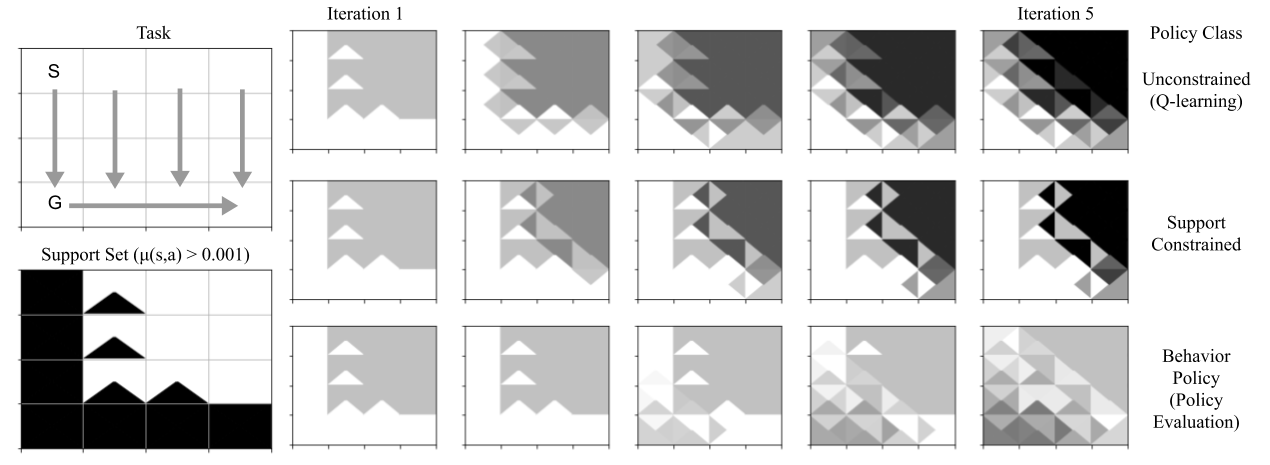
\includegraphics[width=0.9\textwidth]{images/gridworld}
    \caption{Visualized error propagation for various choices of the constraint set $\Pi$
    - unconstrained (AVI,
    %%SL.5.22: is AVI ever defined?
    \TODO{Justin: define AVI, or lets call it Q-learning}
    top row), support-constrained (middle),
    and constraining to the behaviour policy (policy-evaluation, bottom). Dark values represent high error and light values represent low error. The task (leftmost image) is to reach the bottom-left corner from the top-left, but the behaviour policy (visualized as arrows in the task image, support shown in black on the support set image) travels to the bottom-right with a small amount of $\epsilon$-greedy exploration. Standard AVI propagates large errors from the low-data regime into the high-data regime, leading to inaccurate value estimates. Policy-evaluation reduces error propagation from low-data regimes but introduces significant suboptimality bias as the data policy is not optimal. A carefully chosen support-constrained backup strikes a balance between these two extremes by confining error propagation to the low-data region while introducing minimal suboptimality bias.}
    \label{fig:gridworld} 
\end{figure}

% \subsection{Choosing Backup Policies for OOD Action Error Reduction}
% \label{sec:choosing_policies}
% Argument in Sec.~\ref{sec:tradeoff} tells us that, with a careful selection of the policy under which the target value is computed, the overall error of value estimates from the optimal value function $\|V^* - V_k\|$ can be reduced. How should we search for a policy that minimizes the overall error? Our choice is to backup from policies which maintain high-support over the action set of the data.
% %%SL.5.22: I think it's not obvious to readers that "policy for the backup" means the distribution over the actions under which the target value is calculated. -- addressed

% To justify this choice,
% %%SL.5.22: What choice? -- choice of backing up from any policy that maintains high support over data.
% we note that the error analysis relies on being able to quantify $\delta_k(s, a)$ (the per-state-action bellman error) for OOD actions. Outside of the support of the data distribution, it is hard to provide guarantees on $\delta_k$. However, when $a$ lies inside the support of the training distribution for a given state $s$, high-capacity function approximators trained with supervised learning are expected to produce a bounded error, given enough samples.
% %Even if they don't produce bounded error on such in-support inputs, techniques such as Prioritized Replay~\cite{Schaul2016PrioritizedER} can be employed to ensure bounded error on all in-support inputs. 
% %Furthermore, often the quantity of interest is the Bellman error weighted by the inverse density of the behaviour policy~\cite{antos07fitted}, which depends only on the support of the behaviour policy and this error metric is the equal for two policies provided they share the same support.
% Therefore, backing up from all actions that have non-negligible support under the training distribution is sufficient (but not necessary) to prevent error accumulation. Hence, we restrict the set $\Pi$
% %%SL.5.22: Did we define \Pi before? since we cut the set backup operator stuff, now this is much harder to follow. Maybe we can bring it back (but call it something else)?
% of policies used for distribution-constrained backups to the set of policies that are supported on the probable regions of the behaviour policy. That is, $\Pi = \{ \pi | \pi( a | s) = 0 \text{ whenever } \beta( a | s) < \epsilon \}$, where $\beta$ is the behavior policy (i.e., the set of policies that have support in the probable regions of the behavior policy). This means that we are allowed to backup from any action distribution supported over the support of the behaviour policy. Previous work~\cite{fujimoto2018off} restricts the choice of actions to be a distribution close to the behaviour policy. 

%%SL.5.22: I don't really understand what the above paragraph is saying. Read literally, it seems to say "prior work does something similar, and in the worst case we are equally bad." That's not very satisfying. Maybe just delete this paragraph, or rephrase if that's not what you meant?
%Now, explain why this does a good job of balancing the terms. Next, we explain how this bound motivates the use of set-constrained backups to reduce accumulation of bootstrapping error. \TODO{explanation about $\delta1$ goes here} -- addressed -- removed this paragraph


% we need to determine how to formulate the appropriate constraint and how to implement so as to back up only values of policies in $\Pi$.
% %%SL.5.20: Rephrase. In order to develop a practical algorithm based on the set-constrained backup, we need to determine how to formulate the appropriate constraint and how to implement so as to back up only values of policies in $\Pi$.
% Intuitively, we would like $\Pi(s)$ for a particular state $s$ to contain only those policies that permit actions within the support of the dataset distribution. Instead of inferring $\Pi$, we use a notion of divergence between the uniform distribution over the support-set of the current policy and the current policy for optimization.  

% %%SL.5.20: Rephrase. Intuitively, we would like $\Pi(s)$ for a particular state $s$ to contain only those policies that permit actions withi
% In order confidence support set perform the $\max$ on the high-over actions from only these policies, we need to define a tractable objective. Instead of inferring the set of policies $\Pi$ we rather resort to specifying a notion of divergence between the set $\mathcal{A}_\varepsilon^\dataset$ and the current policy, $\operatorname{Divergence}(\mathcal{A}^{\mathcal{D}}_{\varepsilon}(s), \pi)$ thereby fitting the problem of inferring $\Pi$ in an optimization setup.
% %%SL.5.20: I don't really understand the above sentence. Try rewriting it to be clearer?
% Next, we move on to presenting our method, which we call \emph{bootstrap error accumulation reduction} (BEAR).


%%%%%%%%%%%%%%%%%%%%%%%%% OLD: Monday 7:30pm%%%%%%%%%%%%%%%
 % \subsection{Reducing Error Propagation via Set-Constrained Backups}
% Next, we explain how this bound motivates the use of set-constrained backups to reduce accumulation of errors. Suppose we are in an off-policy setting training from a static dataset. Let us denote the set of states and actions within the support of the data as $\mathcal{B}_1$ and the set of states outside of support as $\mathcal{B}_2 = (\mathcal{S} \times \mathcal{A}) - \mathcal{B}_1$. 

% When running Q-learning methods, we typically use supervised learning to minimize Bellman error - stanard supervised learning methods will allow us to control the expected loss on $\mathcal{B}_1$, but not on states over $\mathcal{B}_2$. Suppose that we incur a maximum error of $\delta_1$ on in-distribution states within $\mathcal{B}_1$ and a maximum error of $\delta_2$ on out-of-distribution states within $\mathcal{B}_2$.

% % Set-constrained backups will only be successful at error reduction if the overall error incurred by using set-constrained backups is lower in magnitude than the error incurred when using unrestricted backups. We therefore compare bootstrapping error and error incurred due to the set-constrained backups next.

% %Note that intermediate steps in AVI are all supervised learning problems. When using high-capacity function approximators for these supervised learning problems, we are better able to control the projection error $\delta_k$ induced due to bootstrapping from state-action pairs which lie in the high-confidence support set of the training distribution,  whereas the errors incurred due to backups from state-action pairs outside of this distribution are largely unbounded.
% %%SL.5.20: I noticed that nowhere in this analysis do you actually introduce any notation for the training distribution, and instead you use this set notation $\data$ all the time. As I wrote above, this is very problematic. If one of our central claims is that our analysis treats distributions better than Fujimoto, this isn't going to fly. Can you introduce notation for the training *distribution* (i.e., p(something)) and use that throughout?
% %This is because we can, in principle, overfit
% %%SL.5.20: overfit is the wrong word
% %to the state-action pairs lying in this set
% %%SL.5.20: stop using set
% %with powerful function approximators. However, when we bootstrap from actions that are not present 
% %in the high-confidence support of the train distribution, we back up values that can't be controlled.
% %%SL.5.20: use a different term than "can't be controlled" (we back up values that may have unbounded error)
% %To formalize this, let $\mathcal{A}^{\mathcal{D}}_{\varepsilon}(s) \defeq \{ a \in \mathcal{A} |~ \exists \pi \in \Pi,~ \pi(a|s) \geq \varepsilon \}$ 
% %\TODO{sometimes $\Pi$ is a set, sometimes it's a policy}
% %denote the set of action samples
% %%SL.5.20: the set of actions for state $s$? (maybe also remind the reader why we only worry about actions and not states)
% %that will most likely be sampled from the policies in the set $\Pi$. Let the error incurred in the value estimate at states $s$ reached when backing up from $s'$ using action $a \in \mathcal{A}^{\mathcal{D}}_{\varepsilon}(s')$ be $\delta^1(s)$ and let $\delta^2(s)$ be the error when backing up from $s'$ by using $a \notin \mathcal{A}^{\mathcal{D}}_{\varepsilon}(s')$, we can reasonably expect $\delta^1 < \delta^2$. 
% %%SL.5.20: be consistent with ', i.e., use a' for action in s' and a for action in s

% Using set-constrained AVI will allow us to recover an error bound of (using $\norm{\cdot}_{\infty,\mathcal{B}}$ to denote the maximum over a set $\mathcal{B}$):
%  $\lim_{k \to \infty} \norm{V_k - V^*}_{\infty, \mathcal{B}_1} \le \frac{2\gamma }{(1-\gamma)^2}\left(\max_{s \in , k} \delta^1_k(s) + \alpha(\Pi,s)\right) $
% In contrast, naively running unconstrained AVI will guarantee a bound of:
% $\lim_{k \to \infty} \norminf{V_k - V^*} \le \frac{2\gamma }{(1-\gamma)^2}\left(\max_{s, k} \delta^2_k(s)\right)$. 
% %\TODO{again, does this hold w/ fixed dataset?}
% %%SL.5.20: Can you state this as a theorem with a proof in the appendix? Generally tidying up the above paragraph would be a good idea, this is a very important paragraph and it's currently rather messy.

% Therefore, set-constrained algorithms enable us to accumulate error at the more favorable $\delta^1$ rate
% %$\mathcal{S} \times \mathcal{A}^{\mathcal{D}}_{\varepsilon}$,
% %$\mathcal{S} \times \mathcal{A} -\mathcal{S} \times \mathcal{A}^{\mathcal{D}}_{\varepsilon}$
% , at the cost of introducing additional suboptimality bias. Thus, it is beneficial to use set-constrained backups when $\delta^1 + \alpha < \delta^2$. This is a complex trade-off, which depends on the training data, the underlying MDP, and the function approximator. However, in general $\delta^2$ can be arbitrarily high and exceptionally difficult to control, especially with the use of function approximators such as neural networks, as it uses function-approximation outputs at \emph{state-action pairs at which we have little to no data}. 
% In addition, when our training data is close to optimal, we can expect a small suboptimality bias. Thus, we expect set-constrained algorithms to provide significantly better error bounds many practical scenarios.
% %%SL.5.20: Generally a good idea for several of the other coauthors to take a pass over the previous two paragraphs and tighten them up, deleting anything that is unnecessary. These two paragraphs are crucial for the paper to make sense, and esp the last para is currently way too long-winded.


% % %%% SEEMS TOO SUDDENLY COMING
% % In practice, we are better able to control the projection error $\delta$ on states within our training data than those outside. To formalize this tradeoff, assume we partition the state-action space into two sets, $\mathcal{B}_1$, the in-data set, and $\mathcal{B}_2 = (\mathcal{S} \times \mathcal{A}) - \mathcal{B}_1$, the out-of-data set. We assume that we can control projection error as $\delta^1$ on states within $\mathcal{B}_1$ and $\delta^2$ on $\mathcal{B}_2$, with $\delta^1 < \delta^2$.



% %Justin, it is better if you use this version of algorithm for error propagation 
% %$$
% %\begin{aligned} v_{k}=\left(T_{\pi_{k}}\right)^{m} v_{k-1} & \text { (evaluation step) } \\ \pi_{k+1}=\mathcal{G}\left[\left(T_{\pi_{k}}\right)^{m} v_{k-1}\right] &(\text { greedy step }) \end{aligned}
% %$$

% % Let $\mathcal{A}^{\mathcal{D}}_{\varepsilon}(s) \defeq \{ a \in \mathcal{A} | \pi_{data}(a|s) \geq \varepsilon \}$, and $\mathcal{A}^{\pi_{\theta}}_{\varepsilon}(s) \defeq \{ a \in \mathcal{A} | \pi(a|s) \geq \varepsilon \}$ denote the $\varepsilon$-high confidence support sets of the behaviour policy $\pi_{data}$ and the current actor $\pi$ at state $s$. Actions sampled from $\pi_{data}$ and $\pi$ are most likely to come from these sets respectively, and hence actions from these sets will be used to evaluate expectations or greedy maximum for backing up while performing ADP. If $\operatorname{Divergence}(\mathcal{A}^{\mathcal{D}}_{\varepsilon}(s), \mathcal{A}^{\pi_theta}_{\varepsilon}(s))$ is high, then we end up backing up from actions which haven't been updated, for which our Q-function could give arbitrarily overestimated/underestimated values. Also, note that as there is no implicit normalization mechanism on Q-functions as opposed to policies which are probability distributions and must integrate to 1, there is no check on the values of the Q-function approximator. 

% Now, we pose and answer one key question before presenting our approach to the problem. Given a dataset $\dataset$, how do we constrain our backups to only use policies from $\Pi$?
% %%SL.5.20: Rephrase. In order to develop a practical algorithm based on the set-constrained backup, we need to determine how to formulate the appropriate constraint and how to implement so as to back up only values of policies in $\Pi$.
% The possible candidates for $\Pi$ at a particular state $s$ is the set of policies for which the observed action $a$ lies in the high-confidence support.
% %%SL.5.20: Rephrase. Intuitively, we would like $\Pi(s)$ for a particular state $s$ to contain only those policies that permit actions withi
% In order tconfidence support set $equation$.o perform the $\max$ n the high-over actions from only these policies, we need to define a tractable objective. Instead of inferring the set of policies $\Pi$ we rather resort to specifying a notion of divergence between the set $\mathcal{A}_\varepsilon^\dataset$ and the current policy, $\operatorname{Divergence}(\mathcal{A}^{\mathcal{D}}_{\varepsilon}(s), \pi)$ thereby fitting the problem of inferring $\Pi$ in an optimization setup.
% %%SL.5.20: I don't really understand the above sentence. Try rewriting it to be clearer?
% Next, we move on to presenting our method, which we call \emph{bootstrap error accumulation reduction} (BEAR). 


% Section~\ref{sec:set_constrained_backup} presents a quantitative argument for the restricting the action distribution as an approach to solving the out-of-distribution actions problem in ADP by invoking tools from error propagation. In this section, extend that analysis to motivate the design for a practical algorithm for bootstrapping error reduction. We start by noting there is no direct way that the \TODO{(for Justin): Can we refer to the error-prop stuff under this name -- "abstract error model"} presented above can be instantiated in practice, as it involves the quantities $\delta^1$ and $\delta^2$ which are intractable and can only be measured in retrospect. Moreover, the choice of function approximator strongly affects these errors and theoretical properties of neural net function approximators are not fully understood. However, we can use the error propagation to motivate two design choices for the practical algorithm -- namely, (1) constraining to the support of the dataset action-distribution, (2) correcting the policy improvement step in addition to the policy evaluation step.
% %AK. (Question to Sergey:) Do you think (2) is relevent enough to be mentioned?
 
% Firstly, our definition of BEAR-backup restricts the max-backup to a subset of policies $\Pi$. In practical situations, the set of policies $\Pi$ is observed in the form of an action sample $a$ for each state $s$. Possible candidates for $\pi \in \Pi$ thus include policies for which $a$ belongs to the high-support region. \TODO{complete thia argument} 
% Alongside this, both steps of approximate policy iteration -- evaluation and improvement -- are supervised learning problems in themselves, being solved in practice by using powerful function-approximators such that in principle it is possible to model outputs for high-support datapoints of the training distribution to a high-enough degree of precision which prevents error propagation and accumulation from the set of all the high-confidence support actions. Hence, the out-of-distribution actions problem, in practice, manifests as an out-of-high-confidence support problem - i.e. usage of actions that are less likely than a particular chosen threshold, say, $\varepsilon$ under the training distribution for backups can accumulate a lot of error, but actions show high-enough support are good irrespective of the exact proportions of their appearance in the $\dataset$. 
% %AK.05.15: Question to Sergey: What do you think about the above paragraph? Does it seem too vague, and what's a better way of writing it?
% To formalize this notion, let $\mathcal{A}^{\mathcal{D}}_{\varepsilon}(s) \defeq \{ a \in \mathcal{A} | \Pi(a|s) \geq \varepsilon \}$ denote the $\varepsilon$-high confidence support set of the behaviour policy $\Pi$. Actions sampled from $\Pi$ are most likely to belong to these sets respectively, and hence actions from these sets will be used to evaluate expectations or greedy maximum for backing up while performing ADP. If $\operatorname{Divergence}(\mathcal{A}^{\mathcal{D}}_{\varepsilon}(s), \pi_\theta)$ is high, then we end up backing up from actions which haven't been updated, for which our Q-function could output arbitrarily overestimated/underestimated values.

%%%%%%%%%%%%%%%%%%%%%%%%%%%%%%%% COMMENT HERE
%AK.5.15: Note to Sergey: currently this section is written assuming theory corresponding to approximate policy iteration and not approximate value iteration as is currently present in Section 4.
% Secondly, the two components of $\delta^2$, $\epsilon_k$ (error arising due to approximate policy evaluation), and $\epsilon'_k$ (error arising due to approximate greedy maximization) can be analysed in worst case analysis. If we assume that the dataset $\mathcal{D}$ consists of $N$ samples, and the VC-dimension~\cite{} of the policy class $\Pi$ is denoted bby $h$, then the worst-case error accumulation (apart from intrinsic bellman error) in $\epsilon_k$ is $\mathcal{O}\big(V_{max} \sqrt{\frac{\log (N/\delta) }{N} \big)}$, whereas worst case $\epsilon'_k$ is $\mathcal{O} \big( V_{max} \sqrt{\log (N/\delta)} + V_{max} \sqrt{\frac{h \log (N/h) }{N}} \big)$. For more details, we refer the reader to Lemmas 11 and 12 in \cite{bruno2015approximate}. These bounds suggest that the worst case error incurred in the greedy maximization step is higher than the evaluation step for sufficiently rich function class of policies. Hence, in the worst case, errors in policy improvement can compound fast.
%%%%%%%%%%%%%%%%%%%%%%%%%%%%%%%%%%%%%%%%%%%%%%%%%

% From a practical algorithmic standpoint, the discussion above suggests
% that the actor update in the policy-improvement step be made more constrained, especially to the distribution $\Pi$ with less error compounding then. This also naturally leads to backups with restricted action distributions. Secondly, in practice, the algorithm should always stay in the high confidence support of the set of policies that generated the data. We use these insights to develop an algorithm which we present next.

% Let us revisit the error bounds from the abstract error model for the case of Classification Based Modified Policy Iteration (CBMPI)(\cite{bruno2015approximate}) -- which has a similar structure as modern Actor-Critic algorithms. Theorem 8 in \cite{bruno2015approximate} quantifies the error in the approximate policy iteration scheme defined by the abstract model. We revisit the theorem to gain insights about the problem. Let $\epsilon_k$ and $\epsilon'_k$ be instantaneous worst-case errors incurred in the evaluation step and greedy maximization step respectively. That is,
% $\epsilon_k \defeq v_k -\left(T_{\pi_{k}}\right)^{m} v_{k-1}$ and $\epsilon'_k \defeq \max_{\pi'} T_{\pi'} v_{k-1} - T_{\pi_k} v_{k-1}$. Then, the $\rho$-weighted $p$-th norm of the overall error, $v_* - v_{\pi_k}$ satisfies:
% \begin{multline*}
%     \|v* - v_{\pi_k}\|_{p, \rho} \leq 2 \gamma^{m} \sum_{i=1}^{k-2} \frac{\gamma^{i}}{1-\gamma}\left(\mathcal{C}_{q}^{i, i+1, m}\right)^{\frac{1}{p}}\left\|\epsilon_{k-i-1}\right\|_{p q^{\prime}, \mu}+\sum_{i=0}^{k-1} \frac{\gamma^{i}}{1-\gamma}\left(\mathcal{C}_{q}^{i, i+1,0}\right)^{\frac{1}{p}}\left\|\epsilon_{k-i}^{\prime}\right\|_{p q^{\prime}, \mu}+g(k)
% \end{multline*}

% where $\mathcal{C}_{q}^{l, k, m}$ is a concentrability coefficient and is a function of the MDP, with the property that $\mathcal{C}_{q}^{l, k, m} \geq \mathcal{C}_{q}^{l', k, m}$ for $l \leq l'$. (For more details we refer the reader to \cite{bruno2015approximate}). The concentrability coefficient is a function of the MDP, and hence cannot be controlled. It can therefore be argued that the major contribution in this error term comes from the second term, due to $\epsilon'$, as $m \geq 1$. This implies that imperfect policy improvement step is a major component of bootstrapping error. In modern deep RL settings, this means that optimization of the actor/policy towards regions with imperfect Q-values can be disastrous for the algorithm. Hence, one logical starting point for our approach is to constrain the set of actions we backup from. 

% \section{Error Propagation in Actor-Critic vs Q-Learning Algorithms}
% AVI:
% $$
% \left\|V^{*}-V^{\pi_{K}}\right\|_{p, \rho} \leq \frac{2 \gamma}{(1-\gamma)^{2}}\left[\inf _{r \in[0,1]} C_{V I, \rho, \nu}^{\frac{1}{2 p}}(K ; r) \mathcal{E}^{\frac{1}{2 p}}\left(\varepsilon_{0}, \ldots, \varepsilon_{K-1} ; r\right)+\frac{2}{1-\gamma} \gamma^{\frac{K}{p}} R_{\max }\right]
% $$

% API:
% $$
% \left\|Q^{*}-Q^{\pi_{K}}\right\|_{p, \rho} \leq \frac{2 \gamma}{(1-\gamma)^{2}}\left[\inf _{r \in[0,1]} C_{P(B R A E), \rho, \nu}^{\frac{1}{2 p}}(K ; r) \mathcal{E}^{\frac{1}{2 p}}\left(\varepsilon_{0}, \ldots, \varepsilon_{K-1} ; r\right)+\gamma^{\frac{K}{p}-1} R_{\max }\right]
% $$


\section{Bootstrapping Error Accumulation Reduction (BEAR)}
\label{sec:bear}

We now propose a practical actor-critic style algorithm that uses distribution-constrained backups
%%SL.5.22: Did you define set-constrained backups? I think probably the best thing would be to simply bring back the definition.
to reduce accumulation of bootstrapping error.
Our model has two main components. We use ensembles of Q-functions to provide a conservative estimate of the Q-function which is used in policy improvement, and a constraint which will be used for searching over the set of policies $\Pi$, which share the same support as the behaviour policy. Both of these components will appear as modifications of the policy improvement step in actor-critic style algorithms.

We use an ensemble of Q-functions $\hat{Q}_1, \cdots, \hat{Q}_K$ to compute a conservative estimate of the Q-values: $\frac{1}{K} \sum_{i=1}^K \hat{Q}_i (s, a) - \lambda \sqrt{\operatorname{var}_k \hat{Q}_k(s, a)}$, where $\lambda \in \mathbb{R}^+$ is a hyperparameter. %We use this value as a conservative estimate of the Q-function. This can be derived using Cantelli's inequality. 
Then, the policy is updated to maximize the conservative estimate of the Q-values: $$ \pi_{k+1}(s) := \max_{\pi \in \Pi} E_{a \sim \pi(\cdot|s)} [\hat{Q}_{k}(s, a)] - \lambda \sqrt{ \operatorname{var_k}E_{a \sim \pi(\cdot |s) }[\hat{Q}_k(s, a)]}.$$



% Let $\mathcal{F}_t$ be the sigma-algebra generated by the training procedure until iteration $t$, and let $\operatorname{var}_{t} \hat{Q}(s,a) := \mathbb{E}[(\hat{Q}_t(s, a) - \mathbb{E}[(\hat{Q}_t(s, a) | \mathcal{F}_t))^2|\mathcal{F}_t]$
%%SL.5.20: use mbox. And for clarity, it might be good to indicate what the expectation is over (and use [ instead of ( for E so that parens don't get cluttered). Also, what is up with this (s,a) hanging out at the end? do you mean to put (s,a) inside (after \hat{Q})?
% denote the variance of the Q-function $\hat{Q}_t$, at time $t$ during training. Then, for each state-action pair $(s, a)$, 
% ${Pr (\hat{Q}_t \geq \mathbb{E}(\hat{Q}_t|\mathcal{F}_t) + \sqrt{\frac{(1 - \delta) \operatorname{var}_{t} \hat{Q}_t }{\delta}})  \leq \delta}$
%%SL.5.20: can you state in words what this means for the purpose of this section? also, rhetoric-wise, amybe better state as a theorem (it's kind of obvious, but still) and then after say that this is easy to show via Cantelli's inequality or something?

%%SL.5.20: It's not clear what the concentration bound is actually used for.

 %In the above concentration bound, $\mathbb{E}(\hat{Q}_t|\mathcal{F}_t)$ refers to the true Q-value, which can be obtained given no stochasticity in the procedure.


%%SL.5.20: The logical thread here is broken. What are you doing with set divergence? State the issue first, then th e resolution, else it's hard for the reader to follow.
In practice, the behaviour policy $\beta$ is unknown, so we need an approximate way to constrain $\pi$ to $\Pi$. We define a differentiable constraint that approximately constrains $\pi$ to $\Pi$, and then approximately solve the constrained optimization problem via dual gradient descent.  We use the sampled version of maximum mean discrepancy (MMD)~\cite{gretton2012kernel}
%%SL.5.22: Alg names are not capitalized unless they contain proper nouns, put a space after the words and before open paren (I fixed it above, but this issue happens often, please take this comment into account) -- Thanks for pointing this out!
between the unknown behaviour policy $\beta$ and the actor $\pi$ because it can be estimated based solely on samples from the distributions. Given samples $x_1, \cdots, x_n \sim P$ and $y_1, \cdots, y_m \sim Q$, the sampled MMD between $P$ and $Q$ is given by:\\
$$\operatorname{MMD}^2(\{x_1, \cdots, x_n\}, \{y_1, \cdots, y_m\}) = \frac{1}{n^2} \sum_{i, i'} k(x_i, x_{i'}) - \frac{2}{nm} \sum_{i, j} k(x_i, y_j) + \frac{1}{m^2} \sum_{j, j'} k(y_j, y_{j'}).
$$
Here, $k(\cdot, \cdot)$ is any universal kernel. In our experiments, we find both Laplacian and Gaussian kernels work well.
%As the $\operatorname{MMD}$ distance does not depend on the density function of either distribution, minimizing it using samples is a reasonable proxy for enforcing that $Q$ lies inside the support of $P$. This is because, 
Empirically we find that, in the low sample regime, the sampled MMD between $P$ and $Q$ is similar to the MMD between a uniform distribution over $P$'s support and $Q$ (See Appendix~\ref{} for numerical simulations justifying this approach). %We provide some empirical evidence to justify this choice in the appendix using numerical simulations on gaussian distributions.

% and hence, we parameterize the set $\mathcal{A}^{\mathcal{D}}_{\varepsilon}(s)$ as a distribution $\pi_{set}(a|s)$ such that $\mathcal{A}(s) := \mathcal{A}^{\pi_{set}}_{\varepsilon}(s) := \{a \in \mathcal{A} | \pi_{set}(a|s) \geq \varepsilon \}$, in other words, $\mathcal{A}(s)$ is the high-confidence support set of the distribution $\pi_{set}$, and we train for a parametric $\pi_{set}$.
%%SL.5.20: I don't actually understand at this point what you are doing. Are you optimizing a neural net that denotes \pi_set? or something else?

% \paragraph{Deriving the update:} Let $\hat{Q}_k$ be the Q-function at the k-th step of the algorithm. Actor-critic Q-learning algorithms maintain a parameterized policy, $\pi_k$ that is updated towards the maximizing the Q-function.
% %-- $\pi_{k+1}(s) := \max_{\pi \in \Delta_{|S|}} E_{a \sim \pi(\cdot|s)} [\hat{Q}_{k}(s, a)]$. 
% In order to reduce the number of moving parts, we let the actor in this case serve both its regular function of maximizing the Q-function while also constraining the action distribution close to $\mathcal{A}^\dataset_\varepsilon$, which is the the task of $\pi_{set}$. We use the bound derived on Q-values to update the policy in the direction of maximizing a conservative estimate of the true Q-value -- $$ \pi_{k+1}(s) := \max_{\pi \in \Delta_{|S|}} E_{a \sim \pi(\cdot|s)} [\hat{Q}_{k}(s, a)] - \lambda \sqrt{ \operatorname{var_k}E_{a \sim \pi(\cdot |s) }[\hat{Q}_k(s, a)]}$$
% %TODO{may want to mention that this amounts to subtracting a constant times the std, which sounds reasonable}
% We still need to account for the problem of specifying support divergence. In order to enforce this constraint, we use a measure of support matching between the training distribution $\Pi$ and the policy $\pi(\cdot|s)$, which we choose to be a sampled version of the Maximum Mean Discrepancy(MMD) Distance between $\Pi$ and the actor $\pi$. Sampled MMD distance between two probability distributions $P$ and $Q$ is given by, $\operatorname{MMD}(P, Q)$, where $x_1, \cdots, x_n \sim P$ and $y_1, \cdots, y_m \sim Q$ is given by:\\
% $$\operatorname{MMD}^2(\{x_1, \cdots, x_n\}, \{y_1, \cdots, y_m\}) = \frac{1}{n^2} \sum_{i, i'} k(x_i, x_{i'}) - \frac{2}{nm} \sum_{i, j} k(x_i, y_j) + \frac{1}{m^2} \sum_{j, j'} k(y_j, y_{j'})
% $$
% When the number of samples $n$ is an intermediate number (4-10), the above sampled objective can also be approximately considered as a distance between a uniform distribution over the high confidence support set of the distribution $P$ and the distribution $Q$ -- therefore, if trained perfectly, $Q$ should have the same support as $P$. That is, $\operatorname{MMD}(P, Q)$ is a reasonable proxy for $\operatorname{MMD}(\mathcal{U}(\mathcal{A}_{\varepsilon}(P)), Q)$. 
% %\TODO{what does it mean MMD between a set and distribution}
% The expression for $\operatorname{MMD}$ does not use the density function of either distribution, thereby making it suited as an approximate way of support matching.

Putting it all together, the overall optimization problem in the policy improvement step becomes
\begin{multline}
    \label{eqn:policy_update}
   \pi_{k+1}(s) := \max_{\pi \in \Delta_{|S|}} E_{a \sim \pi(\cdot|s)} [\hat{Q}_{k}(s, a)] - \lambda \sqrt{ \operatorname{var_k}E_{a \sim \pi(\cdot |s) }[\hat{Q}_k(s, a)]}\\
   \text{~~s.t.~~} \mathbb{E}_{s \sim \mathcal{D}} [\operatorname{MMD}(\mathcal{D}(s), \pi(\cdot|s))] \leq \varepsilon
\end{multline}
where $\varepsilon$ is an approximately chosen threshold. We choose a threshold of $\varepsilon=0.05$ in all our experiments. 
% We use an ensemble of $M$ Q-functions, $\{Q_{\theta_i} \}_{i=1}^M$ trained on the same data starting from different initializations for modeling $\operatorname{var}(\hat{Q}|\mathcal{F}_{1:t})$, using sample variance of the ensemble. 
The Algorithm is summarized in Algorithm~\ref{algo:bear_ql}.
% $\operatorname{var}(\hat{Q}_k(s, a)) \approx \frac{1}{M} \sum_{i=1}^{M} (\hat{Q}_{\theta_i, k}(s, a) - \bar{Q}_{\theta, k}(s, a))^2$, where $\bar{Q}_{\theta, k}(s, a) = \frac{1}{M} \sum_{i=1}^{M} \hat{Q}_{\theta_i, k}(s, a)$ is the sample mean of the ensemble. 

%AK.05.15: Note to Sergey: this is the actor-critic version, optional depends on results.
% Another variant of the above approach can be where this single policy improvement step can be decomposed into two decoupled steps -- (1) Learning a policy $\pi_{set}$, whose high-confidence set defines the support set $\mathcal{A}_{\varepsilon}(s)$ at a state $s$, by minimizing the sampling error in $\hat{Q}_k$ and accounting for the deviation from the dataset, and then, (2) Learning to maximize the expected Q-function $\hat{Q}_k$ on this set $\mathcal{A}_{\varepsilon}(s)$, in practice obtained by sampling from $\pi_{set}$. In practice, we found using Equation~\ref{eqn:policy_update} working better than the latter approach and hence, we stick to this formulation for our experiments. The overall algorithm is summarized in Algorithm~\ref{alg:q_learning}, and the actor-critic version is described in Algorithm~\ref{alg:actor_critic}.   

\begin{algorithm}[H]

\small
\caption{BEAR Q-Learning}
\label{alg:q_learning}
\begin{algorithmic}[1]
    \INPUT: Dataset $\mathcal{D}$, target network update rate $\tau$, mini-batch size $N$, sampled actions for MMD $n$, minimum $\lambda$
    \STATE Initialize Q-ensemble $\{Q_{\theta_i} \}_{i=1}^{K}$, actor $\pi_{\phi}$, Lagrange multiplier $\alpha$, target networks $\{ Q_{\theta'_i} \}_{i=1}^K$, and a target actor $\pi_{\phi'}$, with $\phi' \leftarrow \phi, \theta'_i \leftarrow \theta_i$
    \FOR{$t$ in \{1, \dots, N\}}
        \STATE Sample mini-batch of transitions $(s, a, r, s') \sim \mathcal{D}$\\
        \textbf{Q-update:}
            \STATE Sample $p$ action samples, $\{a_i \sim \pi_{\phi'}(\cdot|s')\}_{i=1}^p$
            \STATE Define $y = \max_{a_i} [ \lambda \min_{j=1,..,K} Q_{\theta'_j}(s', a_i) + (1 - \lambda) \max_{j=1,..,K} Q_{\theta'_j}(s', a_i)]$
            \STATE $\forall i, \theta_i \leftarrow \arg \min_{\theta_i} (Q_{\theta_i}(s, a) - (r + \gamma y(s, a)))^2$\\
        \textbf{Policy-update:}
        \STATE Sample actions $\{ \hat{a}_i \sim \pi_{\phi}(\cdot | s) \}_{i=1}^{m}$ and $\{ a_j \sim \mathcal{D}(s)\}_{j=1}^{n}$, $n$ preferably an intermediate integer(1-10)
        \STATE Update $\phi$, $\alpha$ by minimizing Equation~\ref{eqn:policy_update} by using dual gradient descent with Lagrange multiplier $\alpha$
        \STATE \textbf{Update Target Networks: } $\theta'_i \leftarrow \tau \theta_i + (1 - \tau)\theta'_i$; $\phi' \leftarrow \tau \phi + (1 -\tau) \phi'$ 
    \ENDFOR
\end{algorithmic}
\label{algo:bear_ql}
\end{algorithm}

To summarize Algorithm~\ref{algo:bear_ql}: The actor is updated towards maximizing the Q-function while still being forced to remain in the valid search space defined by $\Pi$. The Q-function uses actions sampled from the actor to then perform set-constrained Q-learning, over a reduced set of policies. The maximization step in the actor-update empirically helps, but can be coupled with maximization in Step 5. Similar to \cite{fujimoto2018off} we use a soft-minimum to compute target values for updating Q-functions. Implementation and other details are present in Appendix ?.
%%SL.5.22: Remember to fill this in.

% \begin{algorithm}[H]
% \small
% \caption{BEAR Actor-Critic}
% \label{alg:actor_critic}
% \begin{algorithmic}[1]
%     \INPUT: Dataset $\mathcal{D}$, target network update rate $\tau$, mini-batch size $N$, sampled actions for MMD $n$, minimum $\lambda$, policy gradient clipping constants $\beta_1, \beta_2; \beta_1 \leq \beta_2$, MMD threshold constant $\varepsilon$
%     \STATE Initialize Q-ensemble $\{Q_{\theta_i} \}_{i=1}^{M}$, actor $\pi_{\phi}$, set-determining policy $\pi_{set}$, Lagrange multiplier $\alpha$, target networks $\{ Q_{\theta'_i} \}_{i=1}^M$, and a target actor $\pi_{\phi'}$, with $\phi' \leftarrow \phi, \theta'_i \leftarrow \theta_i$
%     \FOR{$t$ in \{1, \dots, N\}}
%         \STATE Sample mini-batch of transitions $(s, a, r, s') \sim \mathcal{D}$\\
%         \textbf{Q-update:}
%             \STATE Sample $m$ action samples, $\{a_i \sim \pi_{\phi'}(\cdot|s')\}_{i=1}^n$
%             \STATE Define $y = \frac{1}{m} \sum_{a_i} [ \lambda \min_{j=1,..,M} Q_{\theta'_j}(s', a_i) + (1 - \lambda) \max_{j=1,..,M} Q_{\theta'_j}(s', a_i)]$
%             \STATE $\forall i, \theta_i \leftarrow \arg \min_{\theta_i} (Q_{\theta_i}(s, a) - (r + \gamma y))^2$\\
%         \textbf{Set-update and Actor-update:}
%         \STATE Sample actions $A_1(s) \equiv \{ \hat{a}_i \sim \pi_{set}(\cdot | s) \}_{i=1}^{m}$ and $A_2(s) \equiv \{ a_j \sim \mathcal{D}(s)\}_{j=1}^{n}$, $n << m$
%         \STATE Update $\pi_{set}, \alpha$: $$ \pi_{set}, \alpha \leftarrow \arg \min_{\pi_{set}} \max_{\alpha \geq 0} \sqrt{\frac{(1 - \delta) \operatorname{var_k}E_{a \sim \pi_{set}(\cdot |s) }[\hat{Q}_k(s, a)]}{\delta}} + \alpha \mathbb{E}_{s \sim \mathcal{D}} ([\operatorname{MMD}(A_1, A_2)] -  \varepsilon) $$
%         \STATE Update $\phi$ using Importance Sampled Policy Gradient: 
%         $$ \pi_{\phi} \leftarrow  \max_{\pi_{\phi}} \mathbb{E}_{s \sim \mathcal{D}} \mathbb{E}_{a \sim \pi_{set}(\cdot|s)} \Big( \Big[ \frac{\pi_\phi(a|s)}{\pi_{set}(a|s)} \Big]_{\beta_1}^{\beta_2} Q(s, a) \Big)$$
%         \STATE \textbf{Update Target Networks: } $\theta'_i \leftarrow \tau \theta_i + (1 - \tau)\theta'_i$; $\phi' \leftarrow \tau \phi + (1 -\tau) \phi'$ 
%     \ENDFOR
% \end{algorithmic}
% \end{algorithm}


% Let $\bar{Q}(\cdot, \cdot)$ be the delayed target network, and $Q(\cdot, \cdot)$ be the current Q-function. Define $d_i$ be the the TD error for the $i^{th}$ datapoint.
% $$
% d_{i}(Q ; \bar{Q}, \pi)=R_{t}+\gamma \bar{Q}\left(s'_{i}, \pi_{set} \left(s'_i\right)\right)-Q\left(s_{i}, a_{i}\right)

% $$
% Further we define the empirical loss function by
% $$
% \hat{L}_{N}(Q ; \bar{Q}, \pi)=\frac{1}{N} \sum_{t=1}^{N} \frac{d_{t}^{2}(Q ; \bar{Q}, \pi_{set})}{\lambda(\mathcal{A})}
% $$
% where normalization $\lambda{\mathcal{A}}$ is introduced for mathematical convenience. Then, each policy evaluation step can be written as:  

% If we solely backup from actions present in our dataset, there is no way the algorithm can perform better than the policy that collected the data. The capacity of Q-learning and other ADP algorithms to ``stitch'' together performant sub-trajectories is lost. Hence, our method does allow the agent to backup from actions that occur outside the dataset, while still being constrained to not go farther away from the support of $\mathcal{D}$. In principle, a measure of distance from a given dataset can only be obtained using Bayesian Approaches (?). In practice, we use the variance of the ensemble as a measure to approximately quantify closeness to the support set. Our overall approach is described in the next paragraph.




% Our problem setting does not allow any interaction with the environment, and only lets us use the dataset $\mathcal{D}$. Since we see a limited subset of state-action pairs from the environment, the expected estimate of the Q-function conditioned on all training history in our case, $\mathbb{E}(\hat{Q}|\mathcal{F}_t)$, is biased. \TODO{aviral: finish this argument} 

% We train an ensemble of $N$ parametric Q-functions, $Q_{\theta_1}, \cdots, Q_{\theta_N}$ by using bootstrap masks on the data points of the dataset $\mathcal{D}$. This is done to simulate epistemic variance. To make sure that the actions chosen for backing up Q-functions are valid, we learn a set selection policy, $\pi_{set}$ -- a policy that can provide high densities to actions that don't propagate errors.   